\documentclass{article}

% \usepackage[utf8]{inputenc} % Permite escribir caracteres especiales directamente
% \usepackage[spanish]{babel} % Configura el idioma a español

\usepackage{multicol}
\usepackage{tikz}
\usetikzlibrary{automata, positioning}

\title{FULL SAT}
\author{Raudel Alejandro Gómez Molina}

\begin{document}

\maketitle

\section{Lenguaje FULL-SAT}

En esta sección se presentará un nuevo enfoque distinto a los anteriores, el cual se basa en definir un lenguaje al cual
pertenecen todos los problemas SAT que son satisfacible y al cual se le denominará \textit{FULL-SAT}.

\section{Transformación de una fórmula booleana a una cadena}

Primeramente para definir FULL-SAT se debe definir una transformación de una fórmula booleana a una cadena de símbolos.

Dada una fórmula booleana en CNF:
$$F=X_1 \wedge X_2 \wedge \ldots \wedge X_n$$
donde cada cláusula $X_i$ es una disyunción de literales:
$$X_i=L_{i1} \vee L_{i2} \vee \ldots \vee L_{im}$$
y cada literal $L_{ij}$ es una variable booleana o su negación. En cada cláusula $X_i$ las variables que aparecen en $F$,
puede tener cada una 3 estados posibles: $a$ si la variable aparece positiva, $b$ si la variable aparece negada y $c$ si la variable
no pertenece a ninguno de los literales de la cláusula.

Ahora dada la afirmación anterior, se puede definir una cadena de símbolos $w$
que representa a la cláusula $X_i$ sobre una secuencia de variables $v_1,v_2,\ldots,v_p$ de la siguiente manera:

\begin{itemize}
    \item $w$ cuenta con exactamente $p$ símbolos.
    \item Si la variable $v_j$ aparece positiva en $X_i$, entonces el $j$-ésimo símbolo es $a$.
    \item Si la variable $v_j$ aparece negada en $X_i$, entonces el $j$-ésimo símbolo es $b$.
    \item Si la variable $v_j$ no aparece en $X_i$, entonces el $j$-ésimo símbolo es $c$.
\end{itemize}
Si se toma la secuencia de variables correspondiente a $F$, y se le aplica el procedimiento anterior a cada cláusula
se obtendrá una cadena de símbolos que representa a dicha cláusula en $F$.

Si ya se tiene una representación para cada cláusula de $F$ solo resta obtener una cadena de símbolos que represente a $F$,
esto se puede lograr concatenando las cadenas de símbolos de cada cláusula de $F$ en el orden que aparecen con un separador
en este caso se eligió el símbolo $d$.

Por ejemplo la siguiente fórmula booleana en \textit{CNF}:
$$F=(x_1 \vee x_2) \wedge (\neg x_1 \vee x_2 \vee x_3) \wedge (x_1 \vee \neg x_2 \vee x_3)$$
puede ser expresada como la cadena de símbolos:
$$w=aacdbaadabad$$
tomando como secuencia de variables $x_1, x_2, x_3$ como se describió anteriormente.

\subsection{Definición del lenguaje FULL-SAT}

El lenguaje FULL-SAT se define como $L_{FULL_SAT}=\{w\,|\,w \in L_{CNF} \wedge f_{SAT}(w)\}$, donde $L_{CNF}$ representa el lenguaje
de todas las fórmulas booleanas en CNF y $f_{SAT}(w)$ es una función que determinista si $w$ es satisfacible.

En las próximas secciones se presentarán varios enfoques para definir $f_{SAT}$.

\section{Transductor FULL-SAT}

En esta sección la idea para definir $f_{SAT}$ es construir un transductor finito que acepte como entrada cadenas del lenguaje $L_{0,1}=\{wd\}^*$ donde $w\in \{0,1\}^*$
y tenga como salida cadenas, donde cada cadena $e$ representa una fórmula booleana en \textit{CNF} y que acepte si y solo si la fórmula es satisfacible. Detrás
de esta construcción se busca asociar cada carácter 0 ó 1 en la cadena de entrada al valor de la variable booleana correspondiente en la cadena de salida y verificar que para dichos
valores al evaluar la fórmula booleana se obtenga un valor de verdad. Observe que mediante esta construcción se mantiene la invariante fundamental del SAT que a dos instancias
de la misma variable se les asocia el mismo valor de verdad, esto es posible por como está definido el formato de la cadena de entrada.

A continuación se define el transductor finito $T_{FULL-SAT}$ que sigue la construcción definida anteriormente, para ello se define
el transductor $T_{SAT}$ (Figura \ref{fig:transducer}) que hace el proceso de transducción para los valores de verdad de una cláusula $w$, donde $w\in {0,1}$:

\[
    T_{SAT} = (Q_{SAT}, {\Sigma}_{SAT}, \Gamma_{SAT}, \delta_{SAT}, q_{0_{SAT}}, F_{SAT}),
\]
donde:
\begin{itemize}
    \item \(Q_{SAT}\) = ${q_0,q_p,q_n}$.
    \item \(\Sigma_{SAT}\) = ${0,1}$.
    \item \(\Gamma_{SAT}\) = ${a,b,c}$.
    \item \(\delta_{SAT}: Q \times \Sigma \to Q \times \Gamma^*\) función de transición.
    \item \(q_{0_SAT} = q_0\) estado inicial.
    \item \(F={q_p}\) conjunto de estados finales.
\end{itemize}
se define la función de transición $\delta$ de la siguiente manera:

\begin{itemize}
    \item  transiciones para el estado $q_0$: representa el estado inicial.
          \begin{multicols}{2}
              \begin{itemize}
                  \item $\delta_{SAT}(q_0,1)=(q_p,a)$
                  \item $\delta_{SAT}(q_0,0)=(q_n,a)$
                  \item $\delta_{SAT}(q_0,1)=(q_n,b)$
                  \item $\delta_{SAT}(q_0,0)=(q_p,b)$
                  \item $\delta_{SAT}(q_0,1)=(q_0,c)$
                  \item $\delta_{SAT}(q_0,0)=(q_0,c)$
              \end{itemize}
          \end{multicols}
          
    \item  transiciones para el estado $q_p$ (estado positivo de $T_{SAT}$): representa que para los valores de verdad de la cláusula obtiene un valor de verdad positivo.
          \begin{multicols}{2}
              \begin{itemize}
                  \item $\delta_{SAT}(q_{p},1)=(q_{p},a)$
                  \item $\delta_{SAT}(q_{p},0)=(q_{p},a)$
                  \item $\delta_{SAT}(q_{p},1)=(q_{p},b)$
                  \item $\delta_{SAT}(q_{p},0)=(q_{p},b)$
                  \item $\delta_{SAT}(q_{p},1)=(q_{p},c)$
                  \item $\delta_{SAT}(q_{p},0)=(q_{p},c)$
              \end{itemize}
          \end{multicols}
          
    \item  transiciones para el estado $q_n$ (estado negativo de $T_{SAT}$): representa que para los valores de verdad la cláusula obtiene un valor de verdad negativo.
          \begin{multicols}{2}
              \begin{itemize}
                  \item $\delta_{SAT}(q_{n},1)=(q_{p},a)$
                  \item $\delta_{SAT}(q_{n},0)=(q_{n},a)$
                  \item $\delta_{SAT}(q_{n},1)=(q_{n},b)$
                  \item $\delta_{SAT}(q_{n},0)=(q_{p},b)$
                  \item $\delta_{SAT}(q_{n},1)=(q_{n},c)$
                  \item $\delta_{SAT}(q_{n},0)=(q_{n},c)$
              \end{itemize}
          \end{multicols}
\end{itemize}

\begin{figure}[h]
    \centering 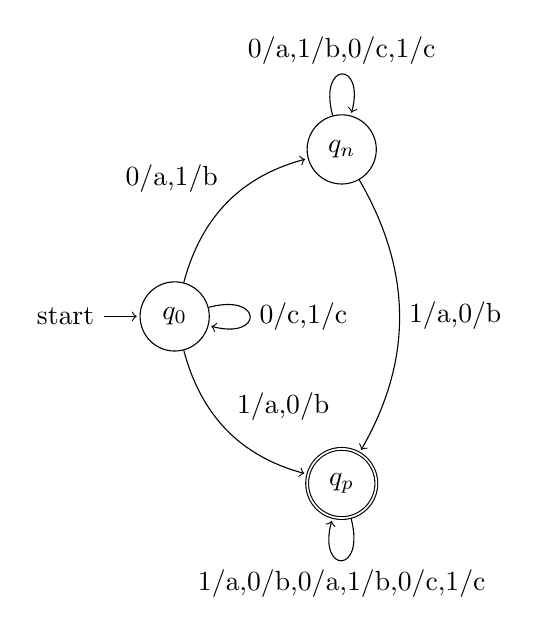
\begin{tikzpicture}[shorten >=1pt, node distance=3cm, on grid, auto]
        
        % Nodos
        \node[state, initial] (q0)   {$q_0$};
        \node[state] (qn) [above right=of q0] {$q_n$};
        \node[state, accepting] (qp) [below right=of q0] {$q_p$};
        
        % Transiciones
        \path[->]
        (q0) edge [bend left] node {0/a,1/b} (qn)
        (q0) edge [bend right] node {1/a,0/b} (qp)
        (q0) edge [loop right] node {0/c,1/c} (q0)
        
        (qn) edge [bend left] node {1/a,0/b} (qp)
        (qn) edge [loop above] node {0/a,1/b,0/c,1/c} (qn)
        
        (qp) edge [loop below] node {1/a,0/b,0/a,1/b,0/c,1/c} (qp);
        
    \end{tikzpicture}
    \caption{Transductor $T_{SAT}$.}
    \label{fig:transducer} % Esto es para referenciar la figura en el texto
\end{figure}

Ahora para definir el transductor $T_{FULL-SAT}$ se toman dos instancias del transductor $T_{SAT}$ ($T_1$ y $T_2$ respectivamente) y se concatenan
añadiendo una transición del estado $q_{p_1}$ (estado positivo de $T_1$) al estado $q_{0_2}$ (estado inicial de $T_2$) con el símbolo $d$ (tanto de
lectura como de escritura) y además se lenguaje agrega una cláusura a $T_2$ con una transición del estado $q_{p_2}$
(estado positivo de $T_2$) al estado $q_{0_2}$ con el símbolo $d$ (tanto de lectura como de escritura). Entonces solo resta definir
el estado inicial y el estado final de $T_{FULL-SAT}$, los cuales serían $q_{0_1}$ (estado inicial de $T_1$) y $q_{0_2}$ (estado inicial de $T_2$),
respectivamente.

\subsection{Definición del lenguaje FULL-SAT usando transducción finita}

Finalmente se define el lenguaje FULL-SAT como el lenguaje de todas las cadenas $e$ que son aceptadas por el transductor $T_{FULL-SAT}$, a partir del lenguaje
de cadenas de entrada $L_{0,1}=\{wd\}^*$ donde $w\in \{0,1\}^*$. 

$$L_{FULL-SAT} = \{e\,|\,\exists w \in L_{0,1} \wedge e \in T_{FULL-SAT}(w) \}$$

Luego $L_{FULL-SAT}$ contiene todas las fórmulas booleanas satisfacibles, pero este conjunto por si solo no sirve de mucho sin un formalismo
que permita conocer si una cadena que representa una fórmula booleana pertenece al lenguaje o no, para ello se necesita encontrar un formalismo que sea capaz
de generar el lenguaje $L_{0,1}$ y al aplicarle el transductor $T_{FULL-SAT}$ a dicho formalismo se obtenga un formalismo que cuente con un algoritmo de parsing
para reconocer si una cadena pertenece a dicho formalismo o no.

\end{document}
